\documentclass{standalone}
\usepackage{tikz}
\usetikzlibrary{patterns, positioning}

\begin{document}
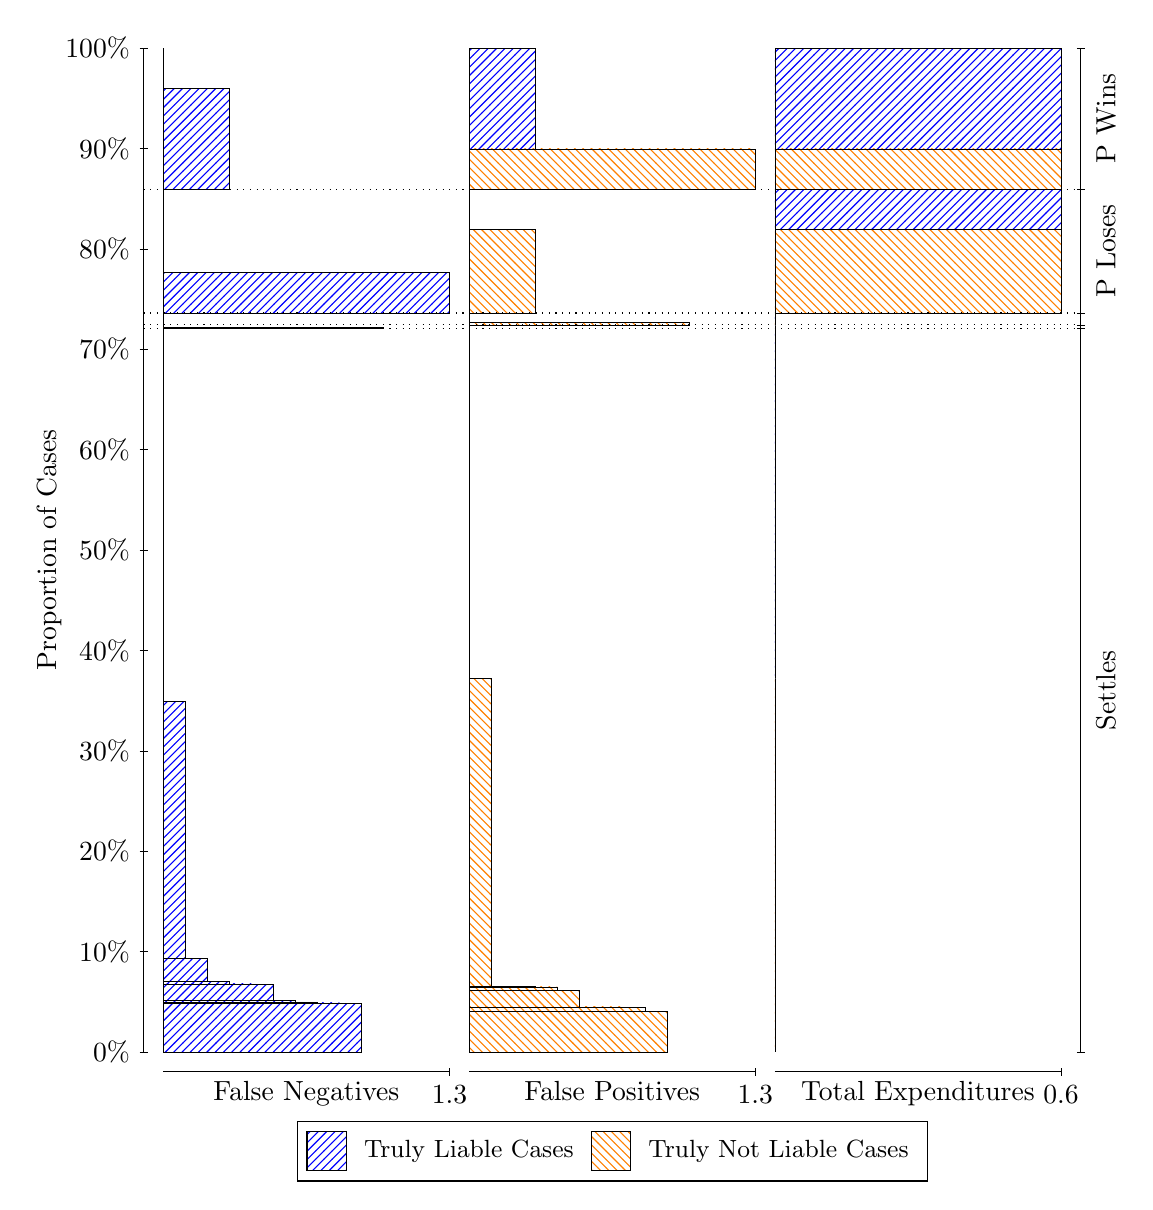
\begin{tikzpicture}
\draw[black, very thin] (1.5,1.75) -- (1.5,14.5);
\node[rotate=90, anchor=center] at (0.3, 8.125) {Proportion of Cases};
\draw[black, very thin] (1.45,1.75) -- (1.55,1.75);
\node[anchor=east] at (1.45, 1.75) {0\%};
\draw[black, very thin] (1.45,3.025) -- (1.55,3.025);
\node[anchor=east] at (1.45, 3.025) {10\%};
\draw[black, very thin] (1.45,4.3) -- (1.55,4.3);
\node[anchor=east] at (1.45, 4.3) {20\%};
\draw[black, very thin] (1.45,5.575) -- (1.55,5.575);
\node[anchor=east] at (1.45, 5.575) {30\%};
\draw[black, very thin] (1.45,6.85) -- (1.55,6.85);
\node[anchor=east] at (1.45, 6.85) {40\%};
\draw[black, very thin] (1.45,8.125) -- (1.55,8.125);
\node[anchor=east] at (1.45, 8.125) {50\%};
\draw[black, very thin] (1.45,9.4) -- (1.55,9.4);
\node[anchor=east] at (1.45, 9.4) {60\%};
\draw[black, very thin] (1.45,10.675) -- (1.55,10.675);
\node[anchor=east] at (1.45, 10.675) {70\%};
\draw[black, very thin] (1.45,11.95) -- (1.55,11.95);
\node[anchor=east] at (1.45, 11.95) {80\%};
\draw[black, very thin] (1.45,13.225) -- (1.55,13.225);
\node[anchor=east] at (1.45, 13.225) {90\%};
\draw[black, very thin] (1.45,14.5) -- (1.55,14.5);
\node[anchor=east] at (1.45, 14.5) {100\%};

\draw[black, very thin] (13.4,1.75) -- (13.4,14.5);
\draw[black, very thin] (13.35,1.75) -- (13.45,1.75);
\node[anchor=west] at (13.35, 1.75) {};
\draw[black, very thin] (13.35,10.94) -- (13.45,10.94);
\node[anchor=west] at (13.35, 10.94) {};
\draw[black, very thin] (13.35,10.984) -- (13.45,10.984);
\node[anchor=west] at (13.35, 10.984) {};
\draw[black, very thin] (13.35,11.135) -- (13.45,11.135);
\node[anchor=west] at (13.35, 11.135) {};
\draw[black, very thin] (13.35,12.706) -- (13.45,12.706);
\node[anchor=west] at (13.35, 12.706) {};
\draw[black, very thin] (13.35,14.5) -- (13.45,14.5);
\node[anchor=west] at (13.35, 14.5) {};

\draw[black, very thin, pattern color=blue, pattern=north east lines] (1.75,1.75) rectangle (4.2654,2.3702);
\draw[black, very thin, pattern color=blue, pattern=north east lines] (1.75,2.3702) rectangle (3.9859,2.3729);
\draw[black, very thin, pattern color=blue, pattern=north east lines] (1.75,2.3729) rectangle (3.7064,2.3756);
\draw[black, very thin, pattern color=blue, pattern=north east lines] (1.75,2.3756) rectangle (3.4269,2.4042);
\draw[black, very thin, pattern color=blue, pattern=north east lines] (1.75,2.4042) rectangle (3.4269,2.4042);
\draw[black, very thin, pattern color=blue, pattern=north east lines] (1.75,2.4042) rectangle (3.1474,2.613);
\draw[black, very thin, pattern color=blue, pattern=north east lines] (1.75,2.613) rectangle (2.8679,2.6138);
\draw[black, very thin, pattern color=blue, pattern=north east lines] (1.75,2.6138) rectangle (2.5885,2.6445);
\draw[black, very thin, pattern color=blue, pattern=north east lines] (1.75,2.6445) rectangle (2.309,2.9383);
\draw[black, very thin, pattern color=blue, pattern=north east lines] (1.75,2.9383) rectangle (2.0295,6.1999);
\draw[black, very thin, pattern color=orange, pattern=north west lines] (1.75,6.1999) rectangle (1.75,10.94);
\draw[black, very thin, pattern color=blue, pattern=north east lines] (1.75,10.94) rectangle (4.5449,10.948);
\draw[black, very thin, pattern color=orange, pattern=north west lines] (1.75,10.948) rectangle (1.75,10.984);
\draw[black, very thin, pattern color=orange, pattern=north west lines] (1.75,10.984) rectangle (1.75,11.011);
\draw[black, very thin, pattern color=blue, pattern=north east lines] (1.75,11.011) rectangle (1.75,11.135);
\draw[black, very thin, pattern color=blue, pattern=north east lines] (1.75,11.135) rectangle (5.3833,11.647);
\draw[black, very thin, pattern color=orange, pattern=north west lines] (1.75,11.647) rectangle (1.75,12.706);
\draw[black, very thin, pattern color=blue, pattern=north east lines] (1.75,12.706) rectangle (2.5885,13.987);
\draw[black, very thin, pattern color=orange, pattern=north west lines] (1.75,13.987) rectangle (1.75,14.5);
\draw[black, very thin, pattern color=orange, pattern=north west lines] (5.6333,1.75) rectangle (8.1487,2.268);
\draw[black, very thin, pattern color=orange, pattern=north west lines] (5.6333,2.268) rectangle (7.8692,2.3154);
\draw[black, very thin, pattern color=orange, pattern=north west lines] (5.6333,2.3154) rectangle (7.5897,2.3223);
\draw[black, very thin, pattern color=orange, pattern=north west lines] (5.6333,2.3223) rectangle (7.3103,2.323);
\draw[black, very thin, pattern color=orange, pattern=north west lines] (5.6333,2.323) rectangle (7.0308,2.5309);
\draw[black, very thin, pattern color=orange, pattern=north west lines] (5.6333,2.5309) rectangle (6.7513,2.5309);
\draw[black, very thin, pattern color=orange, pattern=north west lines] (5.6333,2.5309) rectangle (6.7513,2.5775);
\draw[black, very thin, pattern color=orange, pattern=north west lines] (5.6333,2.5775) rectangle (6.4718,2.5809);
\draw[black, very thin, pattern color=orange, pattern=north west lines] (5.6333,2.5809) rectangle (6.1923,2.5841);
\draw[black, very thin, pattern color=orange, pattern=north west lines] (5.6333,2.5841) rectangle (5.9128,6.4905);
\draw[black, very thin, pattern color=blue, pattern=north east lines] (5.6333,6.4905) rectangle (5.6333,10.94);
\draw[black, very thin, pattern color=orange, pattern=north west lines] (5.6333,10.94) rectangle (5.6333,10.976);
\draw[black, very thin, pattern color=blue, pattern=north east lines] (5.6333,10.976) rectangle (5.6333,10.984);
\draw[black, very thin, pattern color=orange, pattern=north west lines] (5.6333,10.984) rectangle (8.4282,11.011);
\draw[black, very thin, pattern color=blue, pattern=north east lines] (5.6333,11.011) rectangle (5.6333,11.135);
\draw[black, very thin, pattern color=orange, pattern=north west lines] (5.6333,11.135) rectangle (6.4718,12.194);
\draw[black, very thin, pattern color=blue, pattern=north east lines] (5.6333,12.194) rectangle (5.6333,12.706);
\draw[black, very thin, pattern color=orange, pattern=north west lines] (5.6333,12.706) rectangle (9.2667,13.218);
\draw[black, very thin, pattern color=blue, pattern=north east lines] (5.6333,13.218) rectangle (6.4718,14.5);
\draw[black, very thin, pattern color=orange, pattern=north west lines] (9.5167,1.75) rectangle (9.5167,6.4905);
\draw[black, very thin, pattern color=blue, pattern=north east lines] (9.5167,6.4905) rectangle (9.5167,10.94);
\draw[black, very thin, pattern color=orange, pattern=north west lines] (9.5167,10.94) rectangle (9.5167,10.976);
\draw[black, very thin, pattern color=blue, pattern=north east lines] (9.5167,10.976) rectangle (9.5167,10.984);
\draw[black, very thin, pattern color=orange, pattern=north west lines] (9.5167,10.984) rectangle (9.5167,11.011);
\draw[black, very thin, pattern color=blue, pattern=north east lines] (9.5167,11.011) rectangle (9.5167,11.135);
\draw[black, very thin, pattern color=orange, pattern=north west lines] (9.5167,11.135) rectangle (13.15,12.194);
\draw[black, very thin, pattern color=blue, pattern=north east lines] (9.5167,12.194) rectangle (13.15,12.706);
\draw[black, very thin, pattern color=orange, pattern=north west lines] (9.5167,12.706) rectangle (13.15,13.218);
\draw[black, very thin, pattern color=blue, pattern=north east lines] (9.5167,13.218) rectangle (13.15,14.5);
\draw[black, dotted] (1.5,10.94) -- (13.4,10.94);
\draw[black, dotted] (1.5,10.984) -- (13.4,10.984);
\draw[black, dotted] (1.5,11.135) -- (13.4,11.135);
\draw[black, dotted] (1.5,12.706) -- (13.4,12.706);
\draw[black, very thin] (1.75,1.5) -- (5.3833,1.5);
\node[anchor=north] at (3.5667, 1.5) {False Negatives};
\draw[black, very thin] (5.3833,1.45) -- (5.3833,1.55);
\node[anchor=north] at (5.3833, 1.45) {1.3};

\draw[black, very thin] (5.6333,1.5) -- (9.2667,1.5);
\node[anchor=north] at (7.45, 1.5) {False Positives};
\draw[black, very thin] (9.2667,1.45) -- (9.2667,1.55);
\node[anchor=north] at (9.2667, 1.45) {1.3};

\draw[black, very thin] (9.5167,1.5) -- (13.15,1.5);
\node[anchor=north] at (11.333, 1.5) {Total Expenditures};
\draw[black, very thin] (13.15,1.45) -- (13.15,1.55);
\node[anchor=north] at (13.15, 1.45) {0.6};

\node[black, centered, rotate=90] at (13.72, 6.3452) {Settles};


\node[black, centered, rotate=90] at (13.72, 11.921) {P Loses};
\node[black, centered, rotate=90] at (13.72, 13.603) {P Wins};

\draw (7.449999999999999,1.5) node[draw=none] (baseCoordinate) {};
\begin{scope}[align=center]
        \matrix[scale=0.5, draw=black, below=0.5cm of baseCoordinate, nodes={draw}, column sep=0.1cm]{
            \node[rectangle, draw, minimum width=0.5cm, minimum height=0.5cm, pattern=north east lines, pattern color=blue] {}; &
            \node[draw=none, font=\small] (B) {Truly Liable Cases}; &
            \node[rectangle, draw, minimum width=0.5cm, minimum height=0.5cm, pattern=north west lines, pattern color=orange] {}; &
            \node[draw=none, font=\small] (B) {Truly Not Liable Cases}; \\
            };
\end{scope}

\end{tikzpicture}
\end{document}